\chapter{Servicios básicos: UDP y TCP}\label{chap:1}
\section{Programación de red: UDP}
\subsection{Módulos de ayuda}
Para esta práctica, se desarrollan módulos de Python que faciliten las tareas básicas,
como lecturas de hosts y puertos por argumentos: \\
\begin{minipage}{\linewidth}
	\centering
	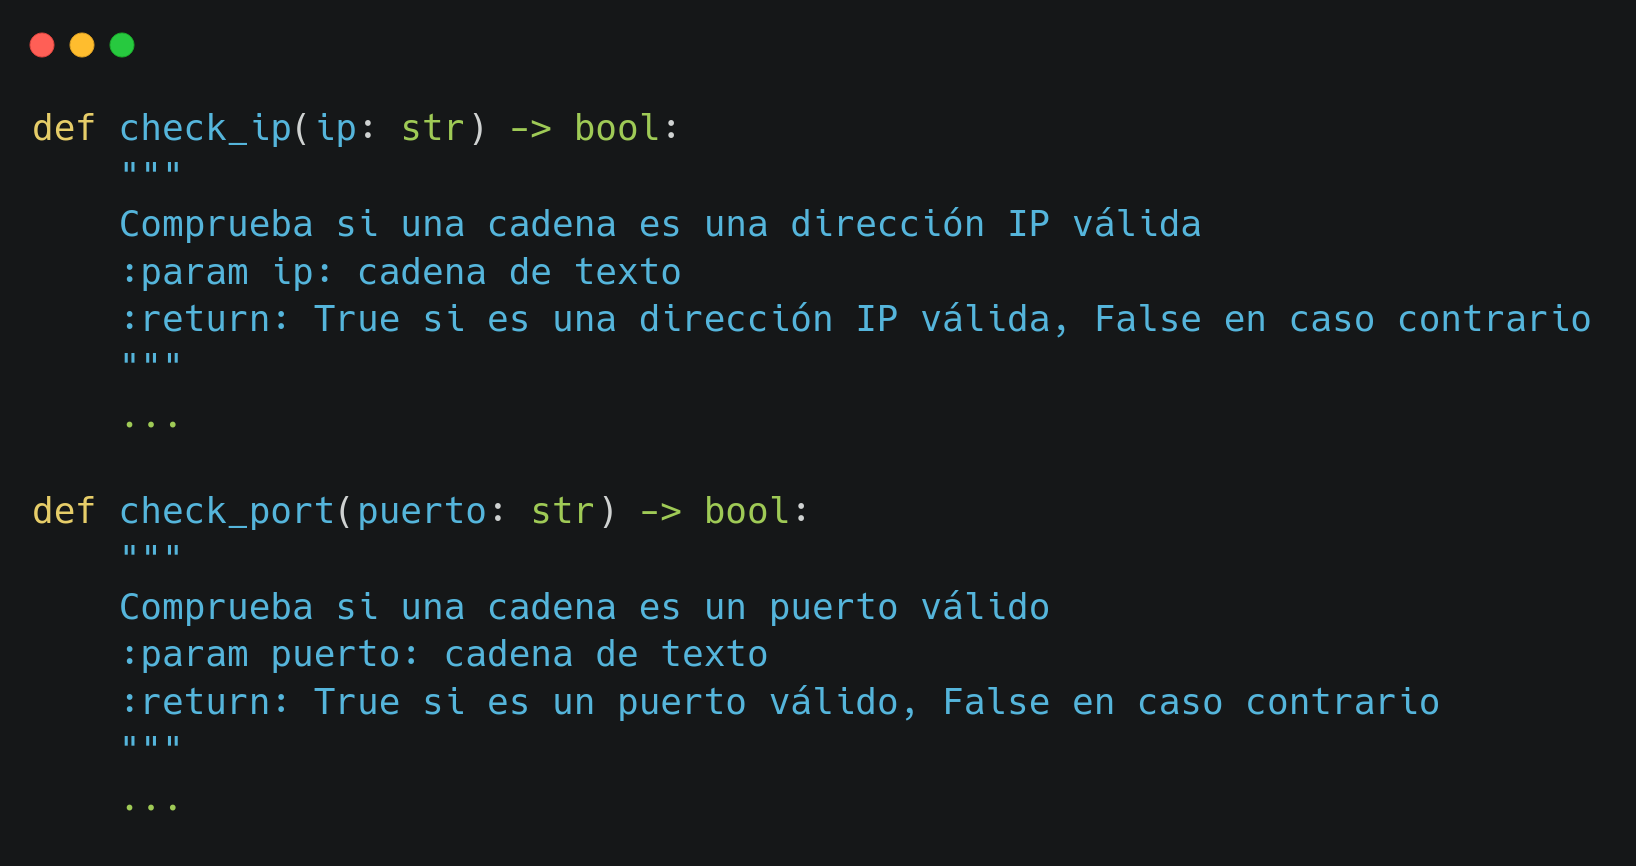
\includegraphics[width=1\textwidth]{1/code1.png}
	\captionof{figure}{Estructura del módulo de ayuda ``ips.py''}\label{fig:1/code1}
\end{minipage}
\\
\begin{minipage}{\linewidth}
	\centering
	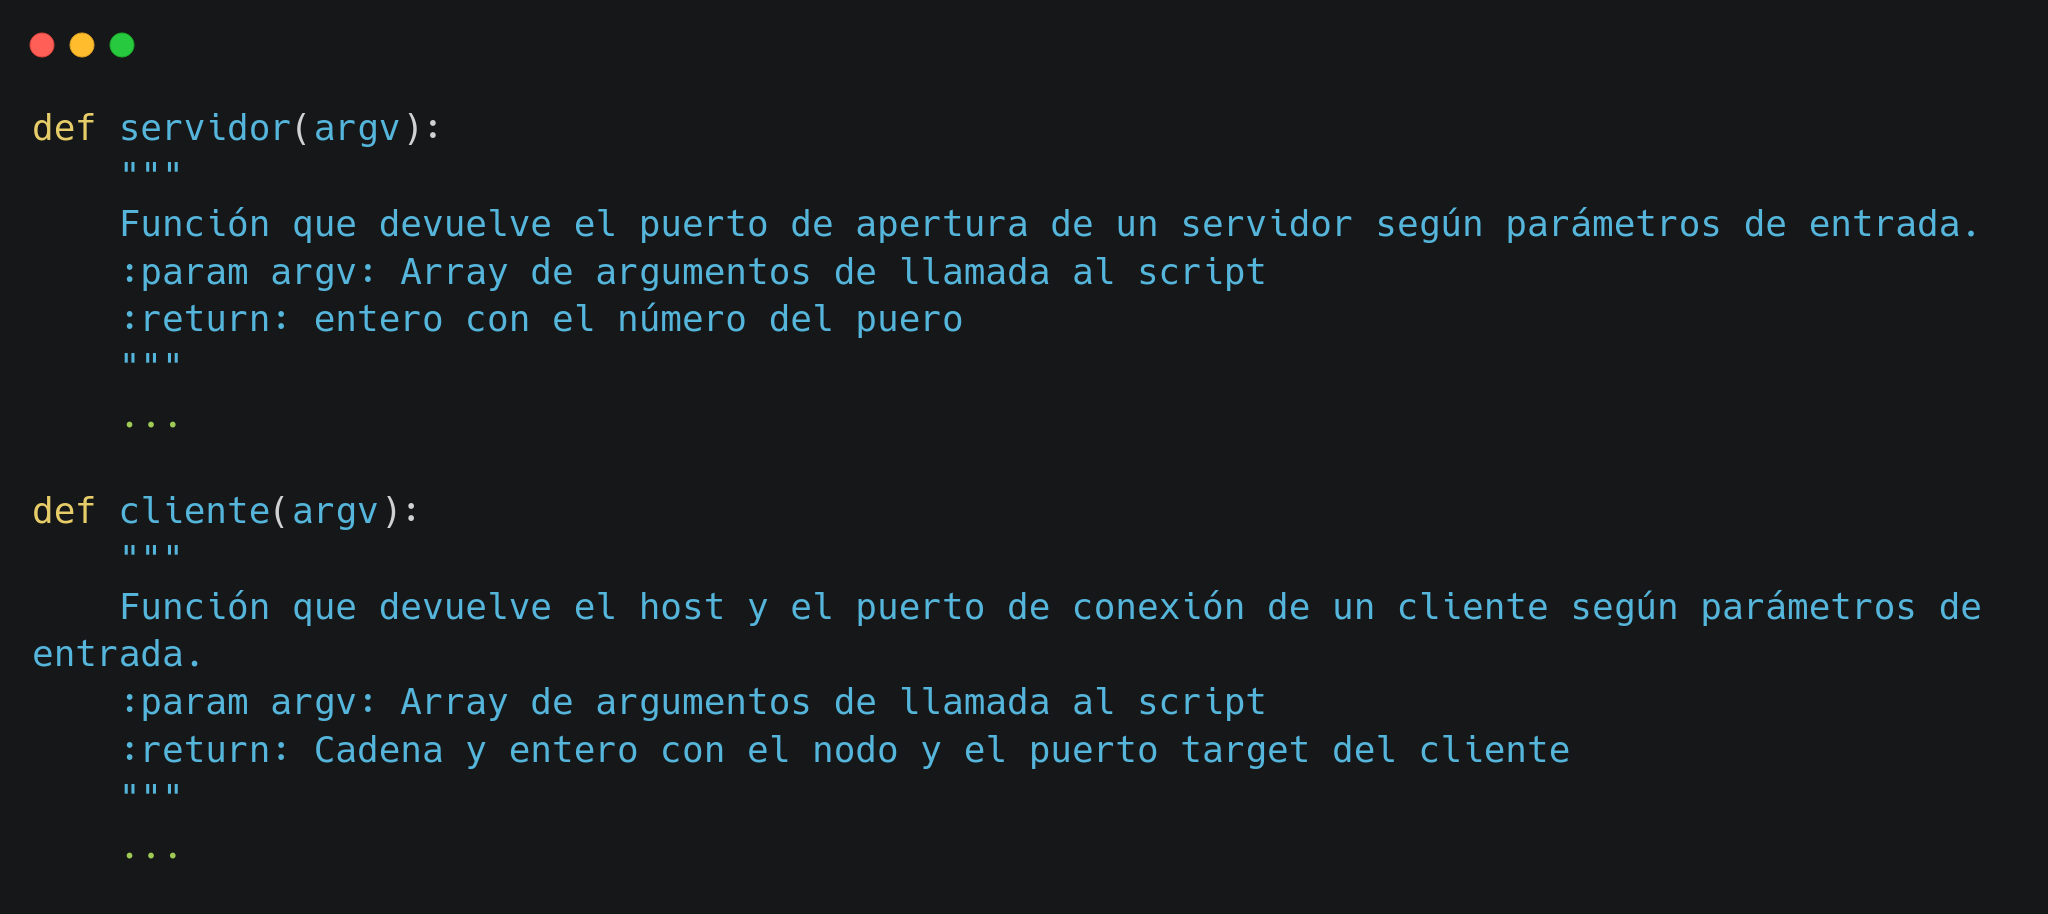
\includegraphics[width=1\textwidth]{1/code2.png}
	\captionof{figure}{Estructura del módulo de ayuda ``ips\_argv.py''}\label{fig:1/code2}
\end{minipage}

\subsection{Ejercicio 1}

El ejercicio solicita que se escriba un servidor que escuche en el puerto indicado por parámetros
o en el 9999 si no se indica ninguno.

El servidor repetirá lo que envien los clientes que se conecten a él.
El cliente se conecta con el servidor y permite al usuario introducir texto que es enviado por el socket.
El cliente finaliza cuando se envía la cadena 'FIN' (esta no se pasa al servidor por el socket).

\subsubsection{udp\_servidor1.py}

\begin{lstlisting}[language=Python]
import socket
import sys

argc: int = len(sys.argv)
port: int = int(sys.argv[1]) if argc >= 2 else 9999

sock: socket.socket = socket.socket(socket.AF_INET, socket.SOCK_DGRAM)
sock.bind(("", port))

print(f"Socket is bind for any address on port {port}")

while (True):
    data, source = sock.recvfrom(1024)
    print(f"Received {data.decode('UTF-8')} from {source}")
sock.close()
\end{lstlisting}

\subsubsection{udp\_cliente1.py}

\begin{lstlisting}[language=Python]
import socket
import sys

argc: int = len(sys.argv)
addr: str = sys.argv[1] if argc >= 2 else 'localhost'
port: int = int(sys.argv[2]) if argc >= 3 else 9999

sock: socket.socket = socket.socket(socket.AF_INET, socket.SOCK_DGRAM)

print(f"Socket is ready to send to addr {addr} on port {port}")
data: str = ""

while (data != 'FIN'):
    data = input("Enter data: ")
    if (data != 'FIN'):
        sock.sendto(data.encode('UTF-8'), (addr, port))
\end{lstlisting}

\subsection{Ejercicio 2}

\subsubsection{udp\_servidor2\_simula\_perdidas.py}

El ejercicio solicita que se modifique el programa del servidor para que simule una pérdida de paquetes
en el 50\percentsign\ de los casos.

En caso de perder un paquete, el servidor imprime por pantalla un mensaje.

\begin{lstlisting}[language=Python]
# ... El inicio del programa es igual al anterior
while (True):
    data, source = sock.recvfrom(1024)
    if (random.randint(0, 1)):
        print(f"Simulating packet loss of {data.decode('UTF-8')} from {source}")
    else:
        print(f"Received {data.decode('UTF-8')} from {source}")
\end{lstlisting}

\subsubsection{udp\_numera2\_numera\_mensajes.py}

El ejercicio solicita que se modifique el programa del cliente para que concatene un número al mensaje.
El número comienza en 1 y se incrementa por cada mensaje que se envía.

\begin{lstlisting}[language=Python]
# ... El inicio del programa es igual al anterior
data: str = ''
idx: int = 1
while (data != 'FIN'):
    data = input('Enter data: ')
    if (data != 'FIN'):
        sock.sendto((f"{idx}: {data}").encode('UTF-8'), (addr, port))
    idx+=1
\end{lstlisting}

\subsubsection{Comprobación}

Esta es la salida del servidor:

\begin{lstlisting}
$ python3 udp\_servidor2\_simula\_perdidas.py
Socket is bind for any address on port 9999
Simulating packet loss of 1: Hi there, sending first message! from ('127.0.0.1', 33252)
Simulating packet loss of 2: Are you getting my messages?? from ('127.0.0.1', 33252)
Received 3: Hello there? from ('127.0.0.1', 33252)
Received 4: There you are! from ('127.0.0.1', 33252)
Received 5: See you later! from ('127.0.0.1', 33252)
\end{lstlisting}

Esta es la salida del cliente:

\begin{lstlisting}
$ python3 udp_cliente2_numera_mensajes.py
Socket is ready to send to addr localhost on port 9999
Enter data: Hi there, sending first message!
Enter data: Are you getting my messages??
Enter data: Hello there?
Enter data: There you are!
Enter data: See you later!
Enter data: FIN
\end{lstlisting}

\subsection{Ejercicio 3}

\subsubsection{udp\_servidor3\_con\_ok.py}

El ejercicio solicita que se modifique el programa del servidor para que envíe un mensaje al cliente
cuando el mensaje es recibido con éxito (cuando no se pierde).

\begin{lstlisting}[language=Python]
# ... El inicio del programa es igual al anterior
while (True):
    data, source = sock.recvfrom(1024)
    if (random.randint(0, 1)):
        print(f"Simulating packet loss of {data.decode('UTF-8')} from {source}")
    else:
        print(f"Received {data.decode('UTF-8')} from {source}")
        sock.sendto("OK".encode('UTF-8'), source)
\end{lstlisting}

\subsubsection{udp\_cliente3\_espera\_ok.py}

El ejercicio solicita que se modifique el programa del cliente para que espere una respuesta del servidor
tras haberle enviado un mensaje.

El cliente esperará una cantidad de tiempo estática a la respuesta del servidor, si no la recibe o
no es la respuesta esperada ('OK') mostrará un mensaje.

\begin{lstlisting}[language=Python]
# ... El inicio del programa es igual al anterior
data: str = ''
idx: int = 1
while (data != 'FIN'):
    data = input('Enter data: ')
    if (data != 'FIN'):
        sock.sendto((f"{idx}: {data}").encode('UTF-8'), (addr, port))
        sock.settimeout(0.1)
        try:
            data, source = sock.recvfrom(1024)
            data = data.decode('UTF-8')
            if (data == 'OK'):
                print("Confirmation received from server")
            else:
                print(f"Malformed confirmation from server received ({data})")
        except socket.timeout:
            print("ERR. No response was received from server")
        except:
            raise
    idx+=1
\end{lstlisting}

\subsection{Ejercicio 4}

\subsubsection{udp\_cliente4\_reintenta.py}

El ejercicio solicita que se modifique el programa del cliente para que reintente el envío del mensaje
si no ha recibido una respuesta del servidor, incrementando el tiempo de espera en cada intento.

En caso que el tiempo de espera exceda los 2 segundos, el programa terminará.
En caso que el programa reciba la respuesta, continuará su curso.

\begin{lstlisting}[language=Python]
# ... El inicio del programa es igual al anterior
data: str = ''
idx: int = 1
while (data != 'FIN'):
    data = input('Enter data: ')
    if (data != 'FIN'):
        success: bool = False
        timeout = 0.1
        while (not success or timeout <= 2.0):
            sock.sendto((f"{idx}: {data}").encode('UTF-8'), (addr, port))
            sock.settimeout(timeout)
            try:
                data, source = sock.recvfrom(1024)
                data = data.decode('UTF-8')
                if (data == 'OK'):
                    print("Confirmation received from server")
                    success = True
                else:
                    print(f"Malformed confirmation from server received ({data})")
            except socket.timeout:
                print("ERR. No response was received from server")
                sys.exit(0)
            except:
                raise
            timeout *= 2
    idx+=1
\end{lstlisting}

\subsubsection{Comprobación}

\subsection{Ejercicio 6}

\subsubsection{udp\_servidor6\_broadcast.py}

El ejercicio solicita que se modifique el programa del servidor para que permita recibir
mensajes de broadcast.

Si recibe el mensaje "BUSCANDO HOLA", responderá a esa IP con el mensaje "IMPLEMENTO HOLA".
Si recibe el mensaje "HOLA", responderá a esa IP con el mensaje "HOLA: \{IP\}".

\begin{lstlisting}[language=Python]
import socket
import sys

argc: int = len(sys.argv)
addr: str = ''
port: int = 12345

sock: socket.socket = socket.socket(socket.AF_INET, socket.SOCK_DGRAM)

sock.setsockopt(socket.SOL_SOCKET, socket.SO_BROADCAST, 1)

print(f"Socket is bind for addr {addr} on port {port}")
sock.bind((addr, port))

while (True):
    data, source = sock.recvfrom(1024)
    data = data.decode('UTF-8')
    print(f"Received {data} from {source}")
    if ("BUSCANDO HOLA" in data):
        sock.sendto("IMPLEMENTO HOLA".encode('UTF-8'), source)
    elif ("HOLA" in data):
        sock.sendto((f"HOLA: {source[0]}").encode('UTF-8'), source)
\end{lstlisting}

\subsubsection{udp\_cliente6\_broadcast.py}

El ejercicio solicita que se modifique el programa del cliente para que pueda enviar mensajes
de broadcast.

Enviará un mensaje "BUSCANDO HOLA" a broadcast, en busca del servidor que implemente este servicio.
Si existe un servidor que lo implemente, el cliente recibirá una respuesta.
El cliente utilizará la dirección IP de esa respuesta para enviar un mensaje "HOLA" a ese servidor.
El servidor responderá y el cliente mostrará su respuesta por la pantalla.
En caso que el cliente reciba varias respuestas de servidores que implementen HOLA, utilizará al primero.

\begin{lstlisting}[language=Python]
import socket
import sys

addr: str = '172.18.0.128' # put bcast addr here
port: int = 12345

sock: socket.socket = socket.socket(socket.AF_INET, socket.SOCK_DGRAM)
sock.setsockopt(socket.SOL_SOCKET, socket.SO_BROADCAST, 1)

sock.sendto("BUSCANDO HOLA".encode('UTF-8'), (addr, port))

addrs = []
is_timeout_alive: bool = True
while (is_timeout_alive):
    sock.settimeout(5)
    try:
        data, source = sock.recvfrom(1024)
        data = data.decode('UTF-8')
        print(f"Received from {source} data {data}")
        if ("IMPLEMENTO HOLA" in data):
            addrs.append(source)
    except socket.timeout:
        print("Timeout")
        is_timeout_alive: bool = False
    except:
        raise

addr = addrs[0]
print(f"Sending to {addr} data HOLA")
sock.sendto("HOLA".encode('UTF-8'), addr)
data, source = sock.recvfrom(1024)
print(f"Received from {source} data {data.decode('UTF-8')}")
\end{lstlisting}

\subsubsection{Comprobación}

\subsection{Ejercicio 7}

El ejercicio solicita que se utilicen los programas escritos previamente en Docker.
Se lanzarán 3 contenedores Docker con el servidor \lstinline{udp\_servidor6\_broadcast.py}
y se lanzará un contenedor Docker con el cliente \lstinline{udp\_cliente6\_broadcast.py}.

El ejercicio indica también que se escriban dos ficheros \lstinline{shell}
que lancen estos contenedores Docker (un \lstinline{shell} para los servidores y otro para el cliente).

\begin{lstlisting}[language=bash]
#! /bin/sh
docker run -it -d --name cliente --network pruebas -v $(pwd):/app python:3.7 python /app/udp_cliente6_broadcast.py
\end{lstlisting}

\begin{lstlisting}[language=bash]
#! /bin/sh
docker run -d --name servidor_0 --network pruebas -v $(pwd):/app python:3.7 python /app/udp_servidor6_broadcast.py
docker run -d --name servidor_1 --network pruebas -v $(pwd):/app python:3.7 python /app/udp_servidor6_broadcast.py
docker run -d --name servidor_2 --network pruebas -v $(pwd):/app python:3.7 python /app/udp_servidor6_broadcast.py
\end{lstlisting}

\section{Programación de red: TCP}
\subsection{Módulos de ayuda}
Se reutilizan los módulos de la sesión anterior (\ref{fig:1/code1}~y~\ref{fig:1/code2}) para
realizar todos los ejercicios. Además, para los ejercicios ``oche'' se reutiliza el código
usando otro módulo nuevo: \\
\begin{minipage}{\linewidth}
	\centering
	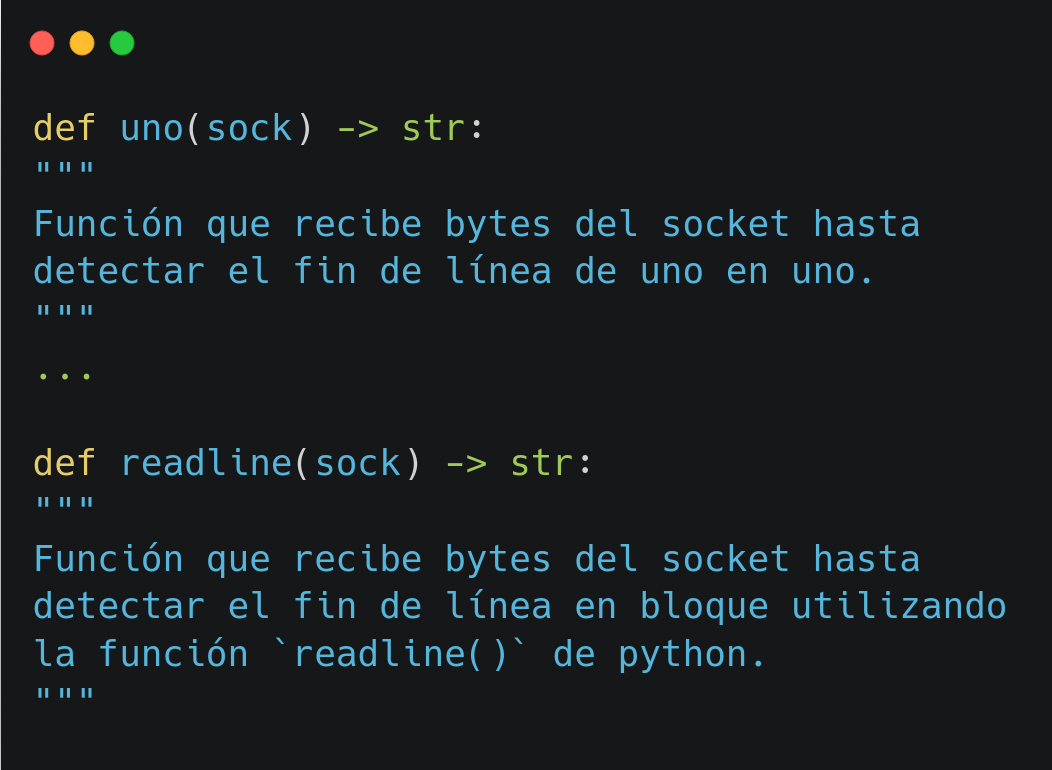
\includegraphics[width=1\textwidth]{1/code3.png}
	\captionof{figure}{Estructura del módulo de ayuda ``recibir\_mensaje.py''}\label{fig:1/code3}
\end{minipage}

\subsection{Ejercicio 1}

\subsection{Ejercicio 2}

\subsection{Experimento}

\subsection{Ejercicio 3 / Experimento}

\subsection{Ejercicio 4 / Experimento}

\subsection{Ejercicio 5}

\subsection{Ejercicio 6}

\subsection{Ejercicio 7 (opcional)}

\subsection{Experimento + Ejercicio Docker}
